Autopilot je sistem sa zatvorenom povratnom spregom unutar sistema za vođenje objekta 
u prostoru koji osigurava da projektil dostigne ubrzanje koje mu sistem vođenja zapovjeda. 
Funkcija autopilota je da stabilizuje i vodi projektil tako što zadaje upravljačke signale kontrolnim 
površinama koji tjeraju projkeil da se rotira ondnosno da translira.  
Pošto tranzijentni odziv projektila varira sa promjenom uslova leta, tako i parametri 
autopilota treba da se mjenjaju sa uslovima leta pa prema tome dobro 
dizajniran autopilot osigurava skoro linearan odziv. Najčešće se za projektovanje 
autopilota koristi linerizirani model drugog reda koji je ranije izveden. 
\section{Upravljanje i stabilizacija ugla propinjanja}
Glavni zadatak autopilota ugla propinjanja je da stabilizuje projektil, tj. da 
da pruži stabilizaciju propinjanja projektila oko longitudinalne ose. Ovo se postiže tako 
što se mjeri brzina propinjnanja i taj signal se koristi da bi se otklonile 
kontrolne površine za iznos koji je potreban da bi se borilo protiv poremećaja. 
Poremećaji u uglu propinjanja mogu nastati zbog atmosferskih porejemćaja ili 
zbog asimetričnosti letjelice. Dalje, često se zahtjeva da ugao propinjanja prati 
određenu referentnu vrijednost. Ovo se može zahtjevati kod "zemlja- zrak" projektila 
kod kojih se zahtjeva da projektil ima isti ugao pri kojem je lansiran sa platforme. 
Viđeno je ranije da odziv ugla propinjanja neograničeno raste na stalan otklon krmila visine 
i da u početku leta ima kratkoperiodične oscilacije. Uvođenjem povratne sprege,
može se postići da ugao propinjanja postigne zadatu stacionarnu vrijednost, ali kratkoperiodične 
oscilacije će i dalje ostati i mogu praviti probleme. Kratkoperiodične 
oscilacije se mogu uklnoiti uvođenjem dodatne povratne sprege po brzini ugla propinjanja 
i time povećati stabilnost procesa. Uvođenjem intgeralnog kompenzatora može se povećati brzina odziva.
U nastavku će se projektovati regulator ugla propinjanja za linerizirani model longitudinalnog kretanja 
koji je dat prenosnom funkcijom:
\begin{equation}
    \frac{\Delta \theta(s)}{\Delta \delta_V(s)}=\frac{K(T_1s+1)}{s(T^2s^2+2\xi Ts+1)}
\end{equation}
Za $K=0.75$, $T_1 = 1s$, $\omega _n = 20 \frac{rad}{s}$ i $\xi = 0.1$. 
Postojenje nule u prenosnoj funkciji uvodi oscilacije i povećava preskok sistema sa 
zatvorenom povratnom spregom. Odziv ugla propinjanja na odskočnu pobudu  je dat na 
slici \ref{fig:propinj}
\begin{figure}[!ht]
    \centering
    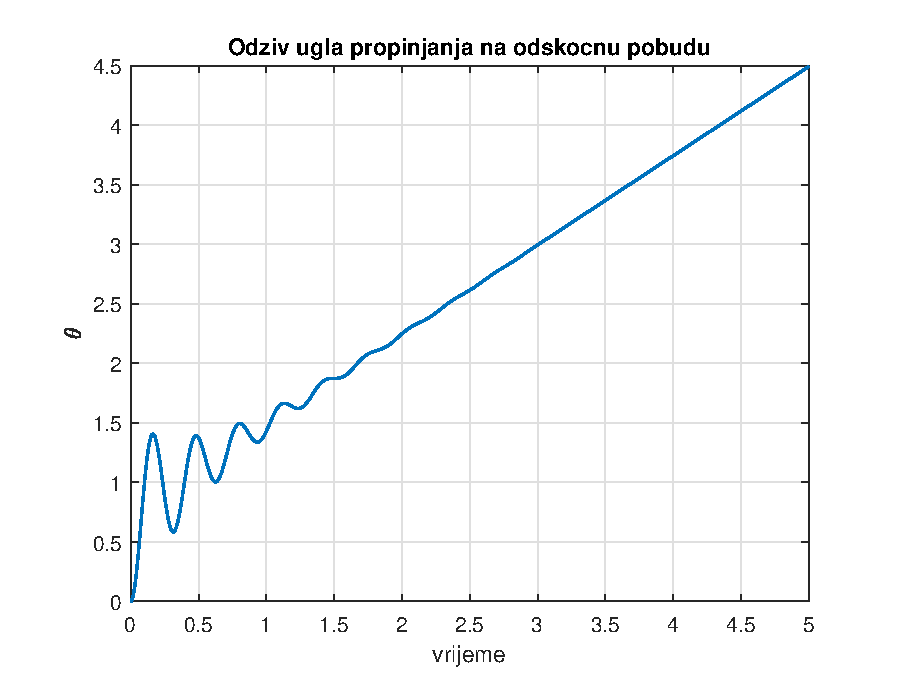
\includegraphics[scale = 0.7]{thetaOtvSprega.eps}
    \caption{Oodziv ugla propinjanja u otvorenoj povratnoj sprezi}
    \label{fig:propinj}
\end{figure} 
Ako se želi da ugao propinjanja prati neku referentnu vrijednost može se uvesti 
povratna sprega po uglu propinjanja preko slobodnog brzinskog žiroskopa. Blok dijagram sistem sa zatvorenom 
povratnom spregom po uglu propinjanja dat je na slici \ref{fig:slobGyro}.
 \begin{figure}[!ht]
     \centering
     \begin{tikzpicture}[auto, node distance=2cm,>=latex']
       \node[input, name=input](input){};
       \node[sum, right of = input](sum){};
       \node[block, right of = sum] (g1){$\frac{K(T_1s+1)}{T^2s^2+2\xi Ts+)}$};
       \node[block, right of = g1,node distance = 2.5cm] (g2){$\frac{1}{s}$};
       \node [output, right of = g2] (output) {};
       \node[block, below of = g1] (gyro){$K_G$};
       \draw [->] (g2) -- node [name=y, anchor = south] {$\theta$}(output);
       \draw[->] (y)|-(gyro);
       \draw[->] (gyro) -|node[pos=0.99] {$-$}(sum);
       \draw[->](g1) -- (g2);
       \draw [draw,->] (input) -- node {$u$} node[pos=0.99] {$+$}(sum);
       \node[anchor = south] (thetadot) at ($(g1)!0.6!(g2)$){$\dot{\theta}$};
       \draw[->] (sum)--(g1);
\end{tikzpicture}
\caption{Povratna sprega po uglu propinjanja}
\label{fig:slobGyro}
\end{figure}
Prenosna funkcija sistema sa zatvorenom povratnom spregom je data sa:
\begin{equation}
    \frac{\theta (s)}{\delta _V(s)} = \frac{\frac{K_GK(T_1s+1)}{T^2s^2+2\xi Ts+)}}{1+\frac{K_GK(T_1s+1)}{T^2s^2+2\xi Ts+)}}
    =\frac{K(T_1s+1)}{T^2s^3+2\xi Ts^2+(1+KK_GT_1)s+KK_G}
\end{equation}
Sada se vidi da je stacionarna vrijednost odziva ugla propinjanja na odskočnu pobudu:
\begin{equation}
    \theta _{stac} = \lim_{s \to 0} s\frac{1}{s}\frac{K(T_1s+1)}{T^2s^3+2\xi Ts^2+(1+KK_GT_1)s+KK_G} = \frac{1}{K_G}
\end{equation}
Odziv ugla propinjanja sa zatvorenom povratnom spregom po uglu propinjanja je data na slici \ref{fig:closedPitch}
\begin{figure}[!ht]
    \centering 
    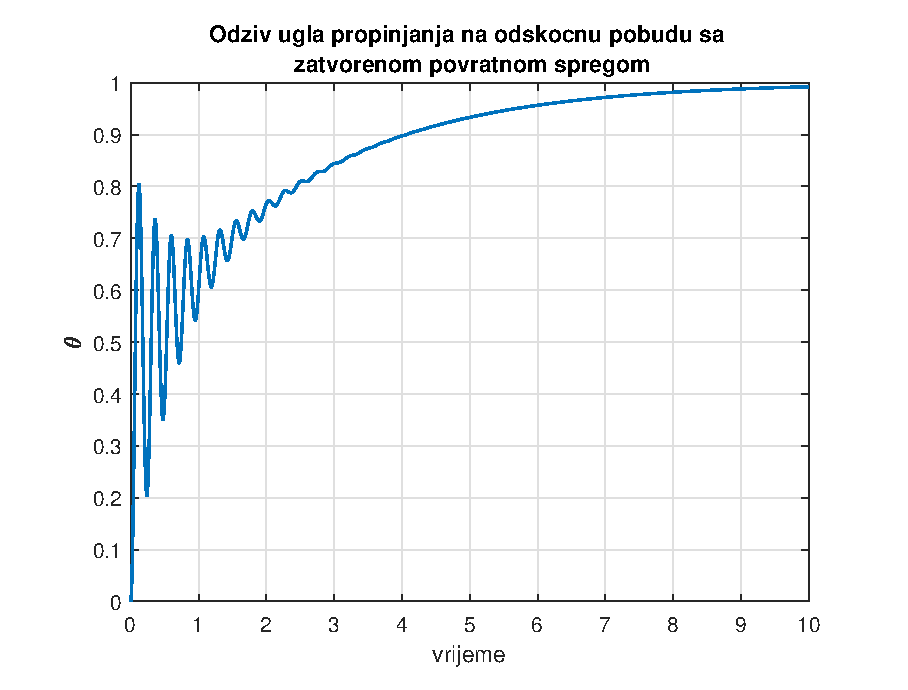
\includegraphics{closedLoopPitch.eps}
    \caption{Odziv ugla propinjanja sa zatvorenom povratnom spregom po uglu propinjanja}
    \label{fig:closedPitch}
\end{figure}
Sada se vidi da se uvođenjem povratne sprege po uglu propinjnja osigurava da ugao propinjanja prati referentnu 
vrijednost, ali se vidi i da je odziv sporiji  i da i dalje postoje kratkoperiodične oscilacije na početku propinjnanja.
Ove oscilacije su posljedica postojanja nule u prenostnoj funkciji zatvorene petlje. 
Uvođenjem integralnog kompenzatora, ova nula se može pokratiti sa polom kompenzatora i tako dobiti glađi odziv.
Uvedimo kompenzator sa prenosnom funkcijom:
\begin{equation}
    G_c(s) = \frac{\alpha T_cs+1}{T_cs+1}  \quad \alpha<1
\end{equation}
Ako se za pol kompenzatora uzme $T_c = T_1$, tada će nula sistema sa otvorenom 
povratnom spregom biti u $-\frac{1}{\alpha T_1}$ što daje veću kontrolu nad postavljanjem 
polova. Povoljnim odabirom parametra $\alpha$ nula se može postaviti na proivoljnu lokaciju.
Odziv sistema sa integralnim kompenzatorom je prikazan na slici \ref{fig:komp}.
\begin{figure}[!ht]
    \centering
    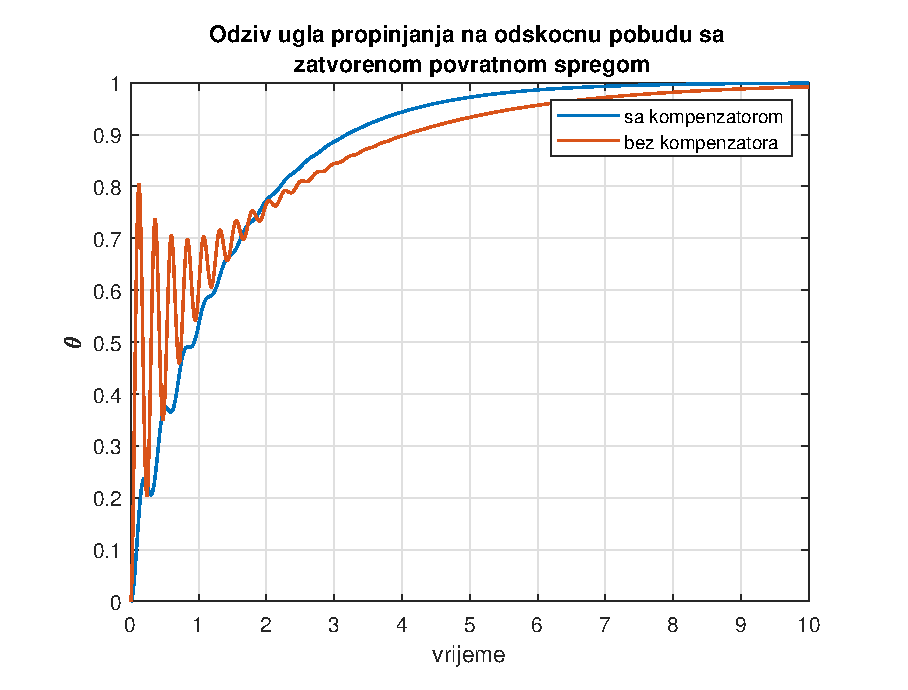
\includegraphics{compareLead.eps}
    \caption{Odziv ugla propinjanja sa integralnim kompenzatorom}
    \label{fig:komp}
\end{figure}
Dodatno, stabilnost odziva se može povećati uvođenjem dodatne povratne sprege po brzini 
ugla propinjanja. Ako se uvede povratna samo po brzini, tada će se stabilizovati samo 
brzina promjene ugla propinjanja a sam ugao propinjanja će imati oblik rampe. 
Blok dijagram ovog upravljačkog sistema je dat na slici \ref{fig:kask}.
\begin{figure}[!ht]
    \centering
    \begin{tikzpicture}[auto, node distance=2cm,>=latex']
        \node[input, name=input](input){};
       \node[sum, right of = input](sum2){};
       \node[sum, right of = sum2](sum){};
       \node[block, right of = sum] (g1){$\frac{K(T_1s+1)}{T^2s^2+2\xi Ts+)}$};
       \node[block, right of = g1,node distance = 2.5cm] (g2){$\frac{1}{s}$};
       \node [output, right of = g2] (output) {};
       \node[block, below of = g1] (gyrosA){$K_{GB}$};
       \node[block, below of = gyrosA, node distance = 1.5cm] (gyro){$K_{GA}$};
       \draw [->] (g2) -- node [name=y, anchor = south] {$\theta$}(output);
       \draw[->] (y)|-(gyro);
       \draw[->] (gyro) -|node[pos=0.99] {$-$}(sum2);
       \draw[->](g1) -- (g2);
       \draw [draw,->] (input) -- node {$u$} node[pos=0.99] {$+$}(sum2);
       \node[anchor = south] (thetadot) at ($(g1)!0.6!(g2)$){$\dot{\theta}$};
       \draw[->] (sum)--(g1);
       \draw[->] (sum2) -- node[pos = 0.99]{$+$}(sum);
       \draw[->] (gyrosA)-| node[pos = 0.99] {$-$}(sum);
       \draw[->] (thetadot)|-(gyrosA);
\end{tikzpicture}
\caption{Povratna sprega po brzini i uglu propinjanja}
\label{fig:kask}
\end{figure}
Vrijednost izvoda ugla propinjanja se dobija pomoću brzinkskog žiroskopa, a 
vrijednost ugla propinjanja se dobija pomoću slobodnog žiroskopa. Pojačanje povratne 
grane iznosi:
\begin{equation}
    H(s)=K_GA+sK_{GB}
\end{equation}
,a pojačanje direktne grane je:
\begin{equation}
    P(s)=\frac{1}{s}\frac{K(T_1s+1)}{T^2s^2+2\xi Ts+)}
\end{equation}
Pa je ukupna funkcija prenosa:
\begin{equation}
    \frac{\theta(s)}{\delta _V(s)} = \frac{K(T_1s+1)}{T^2s^3+
    (2\xi T+KK_{GB}T_1)s^2+(1+KK_{GB}+KK_{GA}T_1)s+KK_{GA}}
\end{equation}
Ovaj sistem je brikazan Simulink blok dijagramomo na slici \ref{fig:simuKask}.
\begin{figure}[!ht]
    \centering
    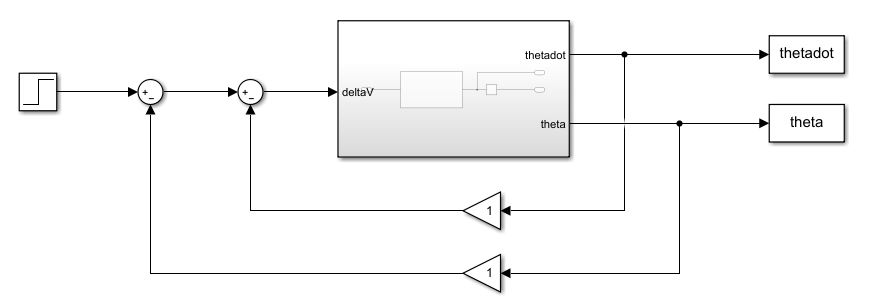
\includegraphics[scale = 0.5]{simKask.JPG}
    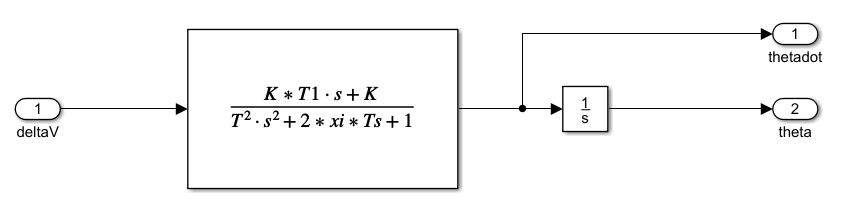
\includegraphics[scale = 0.5]{subKask.JPG}
    \caption{Simulink shema kaskadne regulacije ugla propinjanja}
    \label{fig:simuKask}
\end{figure}
Stacionarna vrijednost na odskočnu pobudu iznosi $\frac{1}{K_{GA}}$
\begin{figure}[!ht]
    \centering
    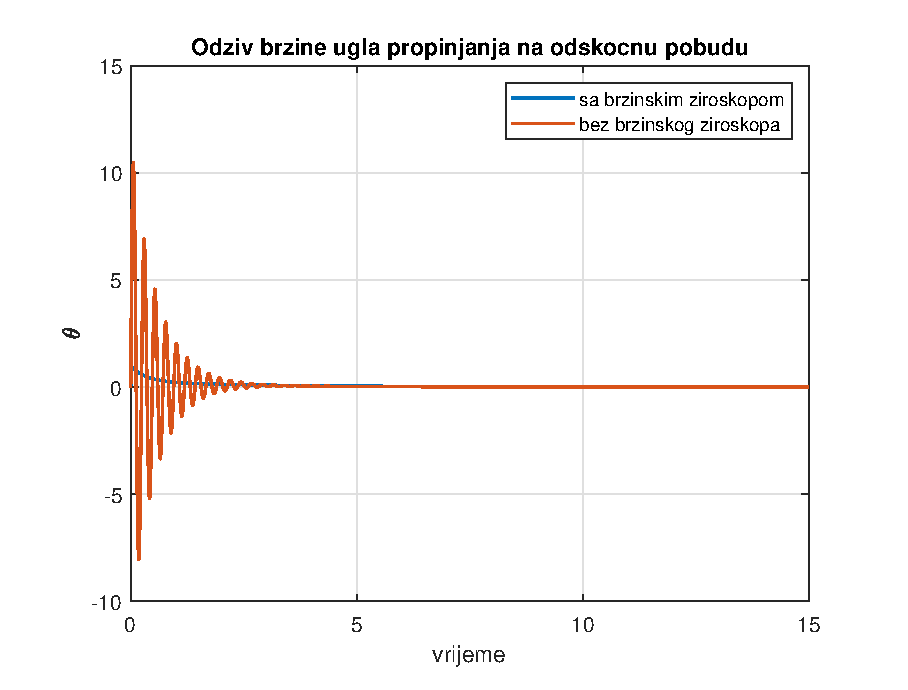
\includegraphics[scale = 0.5]{poredjenjeBrzina.eps}
    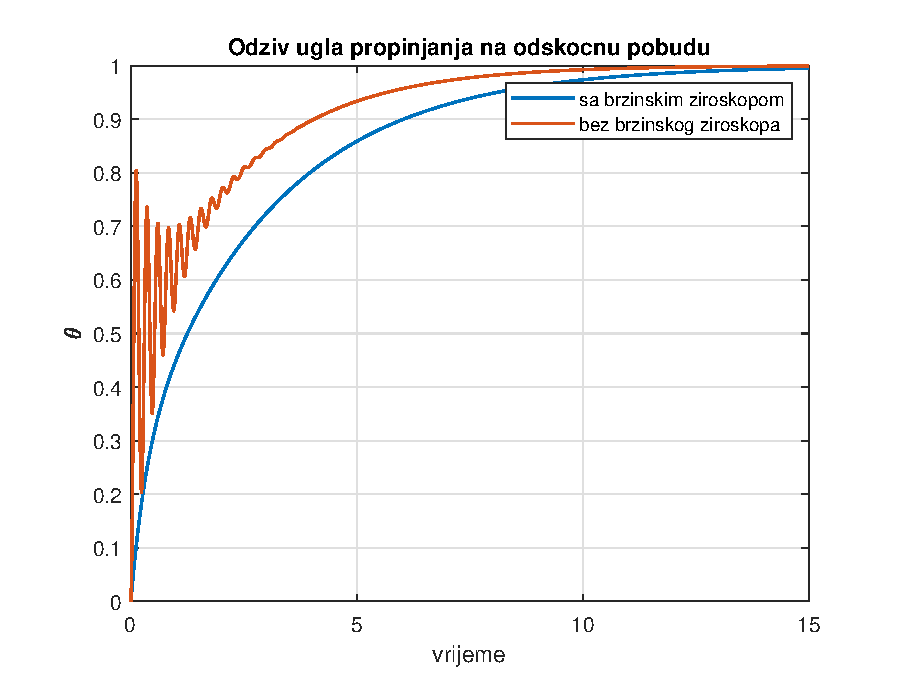
\includegraphics[scale = 0.5]{poredjenjeOdziva.eps}
    \caption{Odzivi ugla propinjanja sa povratnom spregom po brzini i uglu propinjanja}
\end{figure}
%\begin{figure}[!ht]
%    \centering
%    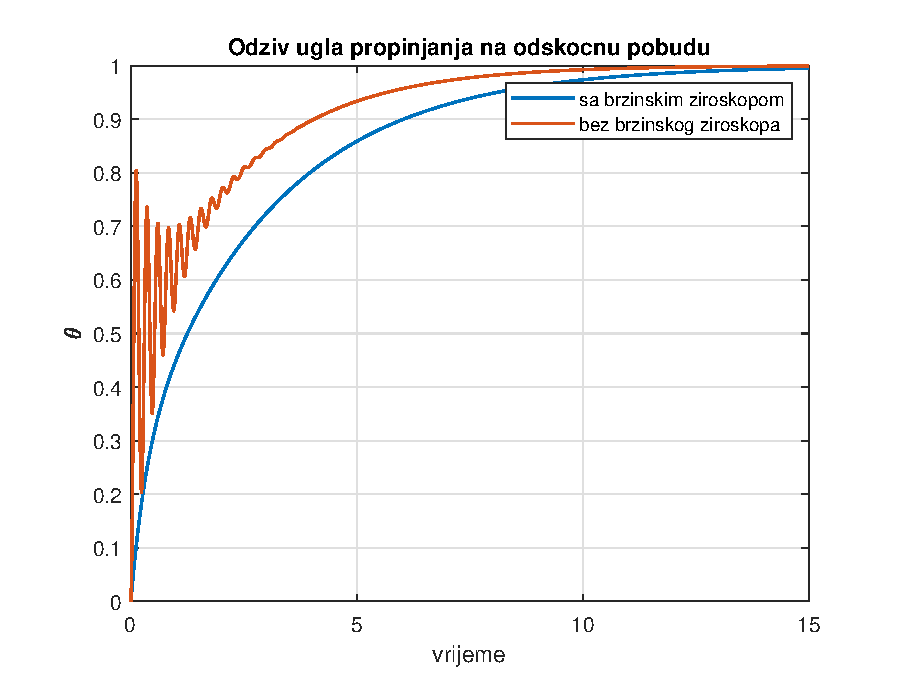
\includegraphics{poredjenjeOdziva.eps}
%\end{figure}
\section{Upravljanje normalnim ubrzanjem}
Kako je razmatrano u prethodnom poglavlju, kod proporcionalne navigacije, se projektilu 
zadaju normalna ubrzanja kako bi on pogodio metu pa je od posebnog interesa imati sitem 
za regulaciju normalnog ubrzanja projektila. Jasno je da će to opet biti upravljanje u 
zatvorenoj povratnoj sprezi. 
\section{Three loop autopilot}